\documentclass{beamer}
%\documentclass[handout]{beamer}

\usetheme[language=english,framenumber,totalframenumber]{AlleghenyCollege}
\usepackage{tikz}

\title{Intelligent Monte-Carlo Tree Search in Perfect Information Games}
\subtitle{Proposal Defense}
\author{Lucas Hawk}
\date{\today}

\begin{document}

\begin{frame}
  \titlepage
\end{frame}

%%%%%%%%%%%% Slide %%%%%%%%%%%%%%%%%%%%%%%%%%%%%%%%%%%%%%%%%%%%%%%%%%%

\begin{frame}
\frametitle{Artificial Intelligence Development and Testing}
\onslide<1-> A major long-term goal of AI research is to develop a system with general intelligence.  How do we move towards this goal?
\begin{itemize}
\onslide<2-> \item Robots
\begin{itemize}
\onslide<3-> \item Expensive and time consuming
\onslide<3-> \item Physical limitations
\end{itemize}
\onslide<4-> \item We need a more testable and controllable environment
\end{itemize}

\end{frame}

\begin{frame}
\frametitle{The Role of Games}
\onslide<1-> Computer games --- specifically perfect information games --- act as a perfect environment.
\begin{itemize}
\onslide<2-> \item Extremely controllable
\onslide<2-> \item Clear goal for players
\onslide<2-> \item Simple programming, complex decision-making
\onslide<2-> \item Easy to benchmark AI against humans
\end{itemize}
\end{frame}

\begin{frame}
\frametitle{Monte-Carlo Tree Search (MCTS)}
\vspace{-0.75in}
\begin{center}
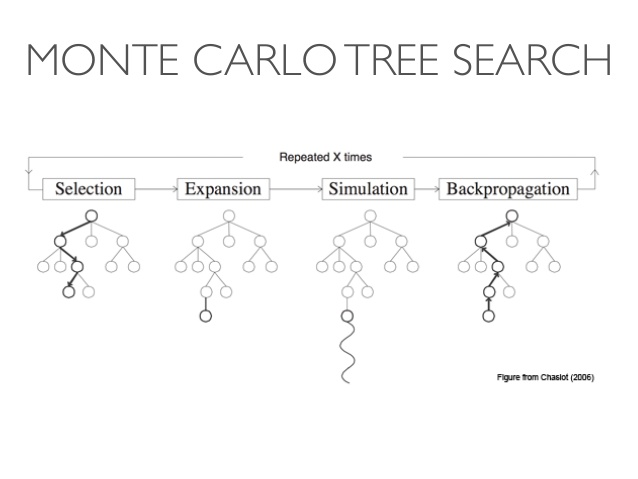
\includegraphics[clip, trim={0 4cm 0 5cm}, scale=.5]{images/mcts.jpg}
\end{center}
\end{frame}

\begin{frame}
\frametitle{Why MCTS?}
\begin{itemize}
\item ``Anytime algorithm''
\item Does not require knowledge of strategy for a game
\item Balances exploration and exploitation
\end{itemize}
\onslide<2-> \[UCT = v_i +C\sqrt{\frac{2\ln N}{n_i}}\]
\onslide<3-> Performance can be enhanced through integration of various AI algorithms
\end{frame}

\begin{frame}
\frametitle{AI Integration}
\vspace{-0.25in}
\begin{center}
Genetic Algorithms\\
\includegraphics[scale=.25]{images/ga1.png}
\end{center}
\end{frame}

\begin{frame}
\frametitle{AI Integration}
\vspace{-0.25in}
\begin{center}
Artificial Neural Networks\\
\def\layersep{2.5cm}

\begin{tikzpicture}[shorten >=1pt,->,draw=black!50, node distance=\layersep]
    \tikzstyle{every pin edge}=[<-,shorten <=1pt]
    \tikzstyle{neuron}=[circle,fill=black!25,minimum size=17pt,inner sep=0pt]
    \tikzstyle{input neuron}=[neuron, fill=black];
    \tikzstyle{output neuron}=[neuron, fill=black];
    \tikzstyle{hidden neuron}=[neuron, fill=black];
    \tikzstyle{annot} = [text width=4em, text centered]

    % Draw the input layer nodes
    \foreach \name / \y in {1,...,4}
    % This is the same as writing \foreach \name / \y in {1/1,2/2,3/3,4/4}
        \node[input neuron, pin=left:Input \#\y] (I-\name) at (0,-\y) {};

    % Draw the hidden layer nodes
    \foreach \name / \y in {1,...,5}
        \path[yshift=0.5cm]
            node[hidden neuron] (H-\name) at (\layersep,-\y cm) {};

    % Draw the output layer node
    \node[output neuron,pin={[pin edge={->}]right:Output}, right of=H-3] (O) {};

    % Connect every node in the input layer with every node in the
    % hidden layer.
    \foreach \source in {1,...,4}
        \foreach \dest in {1,...,5}
            \path (I-\source) edge (H-\dest);

    % Connect every node in the hidden layer with the output layer
    \foreach \source in {1,...,5}
        \path (H-\source) edge (O);

    % Annotate the layers
    \node[annot,above of=H-1, node distance=1cm] (hl) {Hidden layer};
    \node[annot,left of=hl] {Input layer};
    \node[annot,right of=hl] {Output layer};
\end{tikzpicture}
\end{center}
\end{frame}

\begin{frame}
\frametitle{AI Integration}
\vspace{-0.25in}
\begin{center}
Neuro-Evolution\\
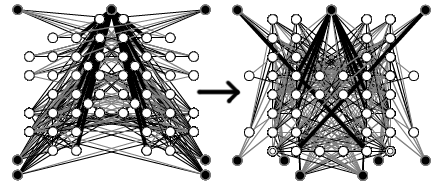
\includegraphics[scale=.75]{images/hyperneatnets2.png}
\end{center}
\end{frame}

\begin{frame}
\frametitle{AI Integration}
\vspace{-0.25in}
\begin{center}
Deep Convolutional Networks\\
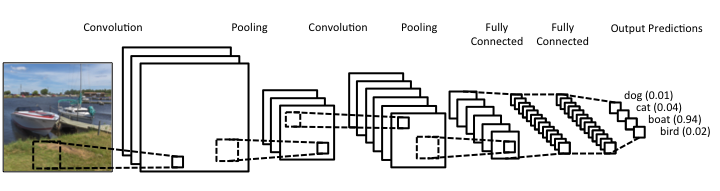
\includegraphics[scale=.4]{images/cnnfull.png}
\end{center}
\end{frame}

\begin{frame}
\frametitle{Existing Implementations}
\begin{itemize}
\onslide<1-> \item Rapid Evolution
\begin{itemize}
\onslide<1-> \item Successful in 99/100 plays of ``Mountain Car''
\end{itemize}
%
\onslide<2-> \item ANN Tree Pruning
\begin{itemize}
\onslide<2-> \item Performs better in 5x5 Go-Moku than standard MCTS --- no specific win-rate given
\end{itemize}
%
\onslide<3-> \item NEAT/HyperNEAT
\begin{itemize}
\onslide<3-> \item HyperNEAT was successful against standard MCTS on 7x7 Go when trained on 5x5 Go
\end{itemize}
%
\onslide<4-> \item AlphaGo
\begin{itemize}
\onslide<4-> \item First program to defeat a professional Go player in a set of 5 games of 19x19 Go
\end{itemize}
\end{itemize}
\end{frame}

\begin{frame}
\frametitle{Our Research}
Provide a direct comparison between these different enhancements of MCTS.
\begin{itemize}
\item Direct competition on several configurations of different games (Go, Hex, Sprouts)
\item Clearly establish differences in performance
\end{itemize}
\end{frame}

\begin{frame}
\frametitle{Experimentation Framework}
Three types of tests
\begin{itemize}
\item Standard experiments --- direct comparison on same games
\item ``Scalability'' experiments --- does training generalize?
\item ``Outperformance threshold'' experiments --- time-per-move doubling experiment
\end{itemize}
\end{frame}

\begin{frame}
\frametitle{In Summary}
\begin{itemize}
\item MCTS is currently the ``golden standard'' for intelligent game-playing agents
\begin{itemize}
\item It can be enhanced through the integration of various AI algorithms
\end{itemize}
\item These different enhancements have not been directly compared
\item We seek to fill this hole in research and highlight the differences in performance through 3 distinct types of experiments
\end{itemize}
\end{frame}

\end{document}